\documentclass[12pt]{article}


\usepackage[english]{babel}


%% Je veux pouvoir inclure des figures...
\usepackage[pdftex]{graphicx}

%% ... des figures ``jpeg'' ou ``pdf'' ou "png"
\DeclareGraphicsExtensions{.jpg,.pdf,.png}

%% Je veux pouvoir inclure gantt diagram...
\usepackage{pgfgantt}

%% Je veux créer des Hyperdocuments
\usepackage[pdftex,colorlinks=true,linkcolor=blue,citecolor=blue,urlcolor=blue]{hyperref}

%% Je contrôle la taille de ma zone imprimée...
\usepackage{anysize}
%% ...en définissants les marges {gauche}{droite}{haute}{basse}
\marginsize{18mm}{18mm}{12mm}{12mm}

%% J'inclue une bibliographie ; j'ai donc besoin du package natbib
\usepackage{natbib}

%Pour utiliser la virgule comme séparateur décimal en mode math,
%sans que Latex introduise un espace inutile après la virgule :
\usepackage{icomma}


\usepackage{minted}

%% pour les referneces
\usepackage{url}


\usepackage{afterpage}

\usepackage{a4wide}
\usepackage{csquotes}
\usepackage{amsmath,amssymb}
\usepackage{bm}
\UseRawInputEncoding
\usepackage[toc,page]{appendix}
\usepackage{color}
\usepackage{captcont}
\usepackage{hvfloat}
\usepackage{siunitx}
\usepackage{forest}
\renewcommand{\figurename}{Fig.}
\usepackage{indentfirst}
\setlength{\parindent}{1cm}

%%\MakeOuterQuote{"}
\oddsidemargin0cm

\topmargin-2cm     %I recommend adding these three lines to increase the 
\textwidth16.5cm   %amount of usable space on the page (and save trees)
\textheight23.5cm 
\usepackage{setspace}
\usepackage[margin=20mm,labelfont=bf]{caption}
\usepackage[left=20mm, right=20mm, top=20mm, bottom=20mm]{geometry}
\usepackage{amssymb}
\usepackage[section] {placeins}
\usepackage{verbatim}
\usepackage{wrapfig}
\usepackage{mwe,tikz,pgfplots}

%% pour les codes 
\usepackage{listings}

\newcommand{\vect}[1]{\hat{\boldsymbol{#1}}}
\title{Report V1}
\author{Congo Job}
\usepackage{minted}
\begin{document}
    \maketitle

\tableofcontents

\section{Introduction}
The regular practice of physical activities has many benefits such as 
as an improvement of mental health, prevention of cardiovascular diseases, limiting weight gain and many others. 

However, we observe a decline in the practice of physical activities.
It appears primordia to encourage young people to maintain a physical activity or to become more active, it is in this optics that this project is registered. 



\subsection{Sport et sciences sociales}

Created in Strasbourg( 1979 ) by Bernard Michon , the Sport and Social Sciences research unit
remains the only STAPS research unit in the Grand Est region and is recognized as a key research structure in the social sciences of sport in France and Europe.
With more than 20 researchers (full and associate) and 17 doctoral students, it produces reference works and articles (more than 174 publications).




\subsection{Main Objectives}

The objective of this work is to identify practitioner profiles based on positive or negative qualifiers, i.e., to assign a profile to each cluster in the data and to estimate the strength of these profiles, i.e., the number of clusters or profiles that are most representative of the data.


\subsection{Specific Objectives}
We will first perform a preprocessing of the data by renormalizing the data, removing outliers, completing or removing missing values, then to analyze the data we will use different algorithms such as: K-means, principal component analysis, decision trees. Finally, we will test the robustness of our cluster by using classification algorithms such as: logistic regression, k-nearest neighbors,...


The Gantt chart below gives us a quick overview of the organization of the work over time.

\begin{ganttchart}[
  hgrid,x unit=1.5mm,
  hgrid style/.style={draw=black!5, line width=.75pt},
  vgrid={*{6}{draw=none},dotted},
  time slot format=little-endian,
]{1-04-2022}{27-05-2022}
  \gantttitlecalendar{ month=shortname,week=4} \\
  \ganttgroup{Report V0}{1-04-2022}{5-04-2022}\\
  \ganttbar{data pre-processing}{5-04-2022}{30-04-2022}\\
  \ganttbar{clustering methods}{5-04-2022}{10-05-2022}\\
  \ganttbar{Validation}{5-04-2022}{22-05-2022}\\
  \ganttgroup{Report V1}{5-04-2022}{22-05-2022}\\
  \ganttbar{data pre-processing}{5-04-2022}{30-04-2022}\\
  \ganttbar{clustering methods}{5-04-2022}{10-05-2022}\\
  \ganttbar{Validation}{5-04-2022}{22-05-2022}\\
  \ganttgroup{Report Vfinale}{22-05-2022}{27-05-2022}\\
\end{ganttchart}



\section{Description of raw data}

The dataset contains personal information about the high school students (1070 participants) such as their initial, high school, gender, study choice, parents' work and parents' support as well as date of birth, body shape (height and weight). Twenty variables measure the nature of motivation such as enjoyment, affiliation, physical condition and the degree of motivation such as SIMS intrinsic and SIMS external regulation. 

Finally, the rest of the variables (71) were collected as follows:
We ask a question: "In PE, what is the sport that you enjoyed the most?

Then we indicate:
"We are now going to present you with words that will allow you to describe how you feel about this sport. Your job is to indicate, as quickly as possible, whether you agree or disagree with these propositions by clicking on yes or no.
The response time has been taken into account in each answer. If this time is short, it means that the term seems obvious.
For example, if the sport is "soccer", the student could answer "yes" quickly to the qualifier "fun", "no" quickly to the qualifier "beauty".

The possible answers to each question are "yes", "no", "I don't know". When the answer to a question is "yes", the time value is positive, negative in the case of "no" and zero in the case of "I don't know".


\begin{figure}[h]
\begin{center}
\includegraphics[scale=0.5]{donnée_brute.png} 
\caption[]{ Raw \ data}
\end{center}
\end{figure}


\section{Preprocessing}

\subsection{Preprocessing Method}

The missing values are set to zero assuming that the qualifier is not of interest to the students concerned and that they could have answered: "I don't know".
For the management of the outliers, those which are higher than 5*standard deviation have been set to zero in order not to impact the weight given to each word. The standard deviation is calculated using the unsigned data in order to reduce the extreme values and avoid the possible compensation of the values.
The students who answered "I don't know" to all these questions were not considered in the rest of the project.  
The normalization is done by line in order to keep what is "important" for each person. 



\subsection{Results of processed data}

\begin{figure}[h]
\begin{center}
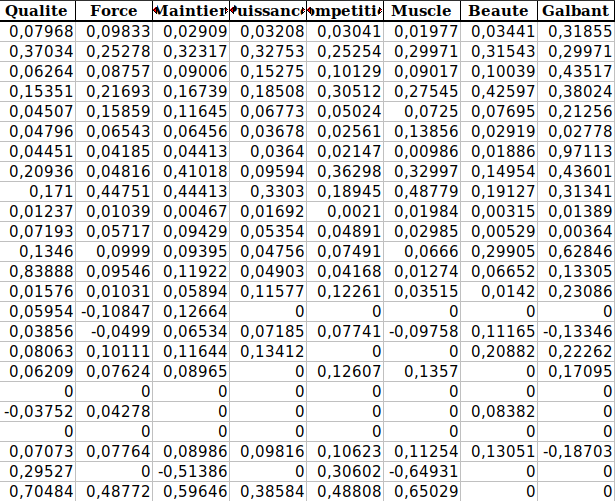
\includegraphics[scale=0.7]{donnée_nettoyé.png} 
\caption[]{Data \ processed }
\end{center}
\end{figure}

The most "important" and least "important" words for each person are respectively close to either 1 or -1 . Those which are less "important" are close to zero.

The cleaned dataset contains 1050
high school students and 71 features.


\section{Clustering} 


\subsection{Principal component analysis}

Principal Component Analysis (PCA) is used to reduce the size of the data to a few variables and keep the most important data. It is a method of multivariate statistics, which consists in transforming variables related to each other (called "correlated" in statistics) into new variables decorrelated from each other. 

To determine the number of optimal components, the function fviz\_eig of Rstudio was used. This function allows to have the graph of the eigenvalues.

The eigenvalues measure the amount of variance explained by each principal axis. They are large for the first axes and small for the following axes.


\begin{figure}[H]
\begin{center}
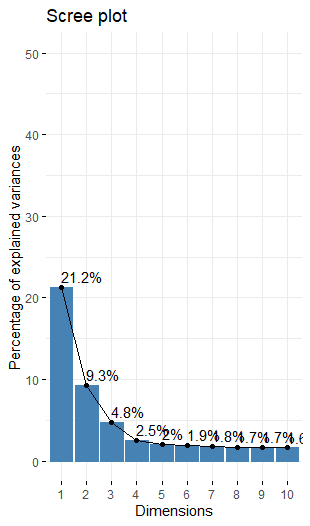
\includegraphics[scale=1.1]{ACP_1.png} 
\caption[]{\ }
\end{center}
\end{figure}

From the graph above, we might want to stop at the fifth principal component because 
stop at the fifth principal component because the variation is less after the fifth.
However 39.79760 \% of the information (variances) contained in the data is retained by the first 5 principal components.
in the data is retained by the first 5 principal components.


The graph below shows the top 30 variables that contribute the most to the 5 principal components. 
The red dotted lines on the graphs indicate the average contribution value.
 

\begin{figure}[H]
\begin{center}
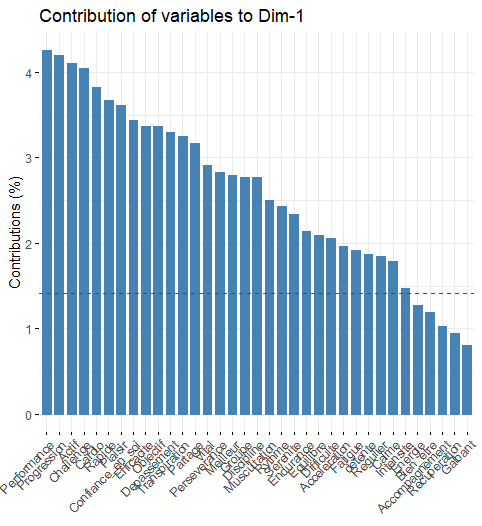
\includegraphics[scale=1.3]{ACP_2.png} 
\caption[]{\ }
\end{center}
\end{figure}


\begin{figure}[H]
\begin{center}
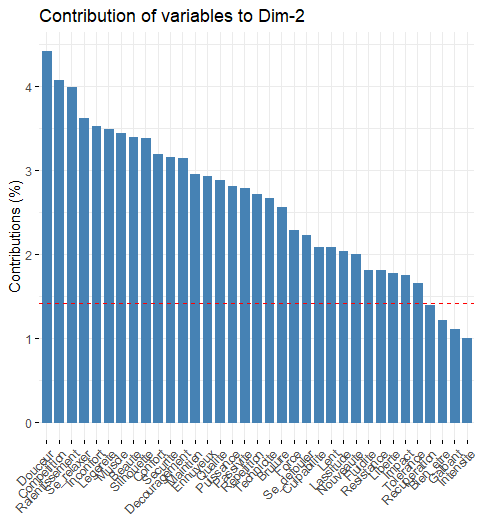
\includegraphics[scale=1.3]{ACP_3.png} 
\caption[]{\ }
\end{center}
\end{figure}


\begin{figure}[H]
\begin{center}
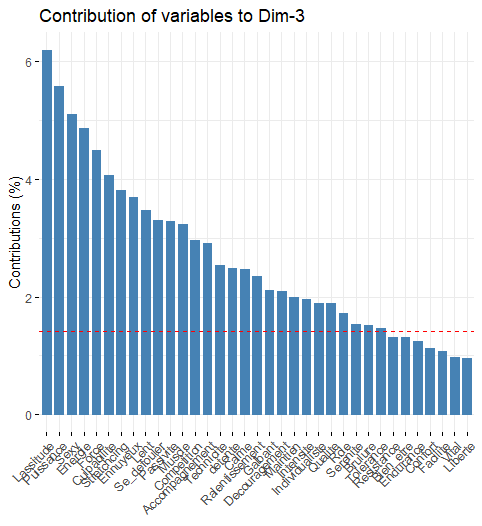
\includegraphics[scale=1.3]{ACP_4.png} 
\caption[]{\ }
\end{center}
\end{figure}


\begin{figure}[H]
\begin{center}
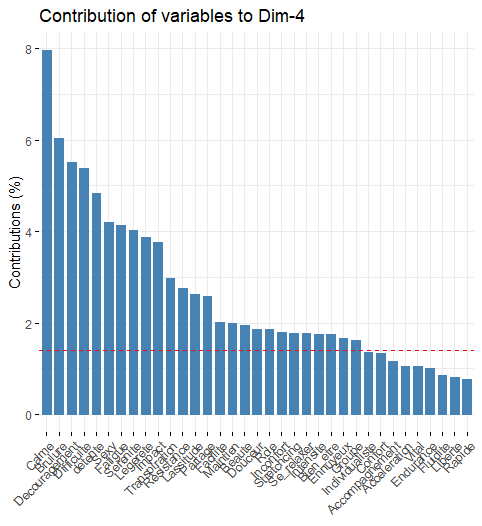
\includegraphics[scale=1.3]{ACP_5.png} 
\caption[]{\ }
\end{center}
\end{figure}


\begin{figure}[H]
\begin{center}
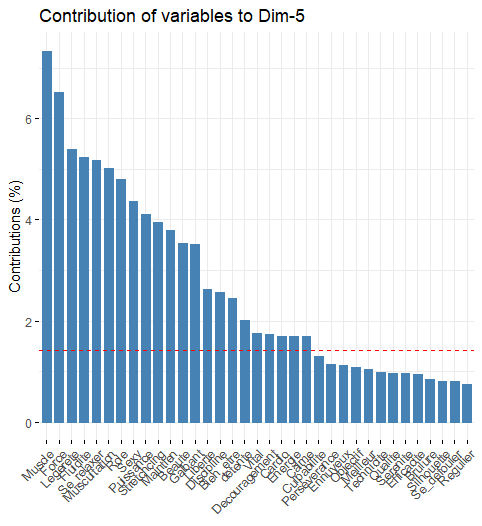
\includegraphics[scale=1.3]{ACP_6.png} 
\caption[]{\ }
\end{center}
\end{figure}

The least important variables are "Recuperation" and "Facilite".

\newpage   


\subsection{Hierarchical Clustering on Principal Components}

To perform the clustering, we will use Hierarchical Clustering on Principal Components (HCPC).
This method combines the three standard methods used in multivariate data analysis:

    
 \begin{itemize}
    \item  Principal component methods (PCA, CA, MCA, FAMD, MFA),
    \item  Hierarchical regrouping and
    \item  Partitioning clustering, in particular the k-means method.
 \end{itemize}

\vspace{0.2 cm}

The HCPC method algorithm has 4 main steps:

\begin{enumerate}
    \item  Perform a PCA. Choose the number of dimensions to retain by specifying the argument ncp. In our case, the value is 5.
    \item Apply the hierarchical classification on the result of step 1.
    \item Choose the number of groups according to the dendrogram obtained in step 2. In our case, the number of groups is 3.
    \item Perform k-means to improve the initial partitioning obtained in step 3.
\end{enumerate}


%% suprimer ligne code ??

Here are the main lines of code in Rstudio for the implementation:

\begin{lstlisting}

res.pca <- PCA(data_base , ncp = 5 ,graph = TRUE)
res.hcpc <- HCPC(res.pca,nb.clust=3,consol=FALSE,graph=TRUE)

plot(res.hcpc,choice = "tree")
plot(res.hcpc,choice = "map", draw.tree = FALSE)
plot(res.hcpc,choice = "3D.map")
catdes(res.hcpc$data.clust,ncol(res.hcpc$data.clust))

\end{lstlisting}



\begin{figure}[H]
\begin{center}
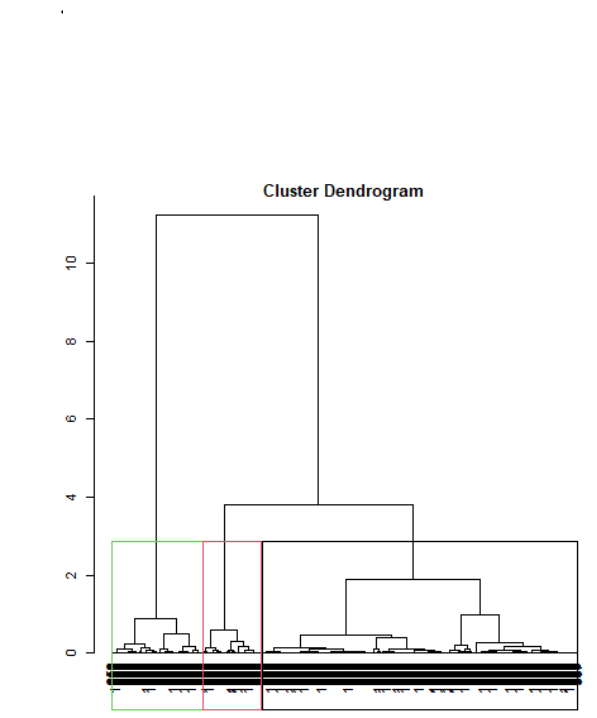
\includegraphics[scale=0.65]{classification_1.png} 
\caption[]{Hierarchical \ tree}
\end{center}
\end{figure}


\begin{figure}[H]
\begin{center}
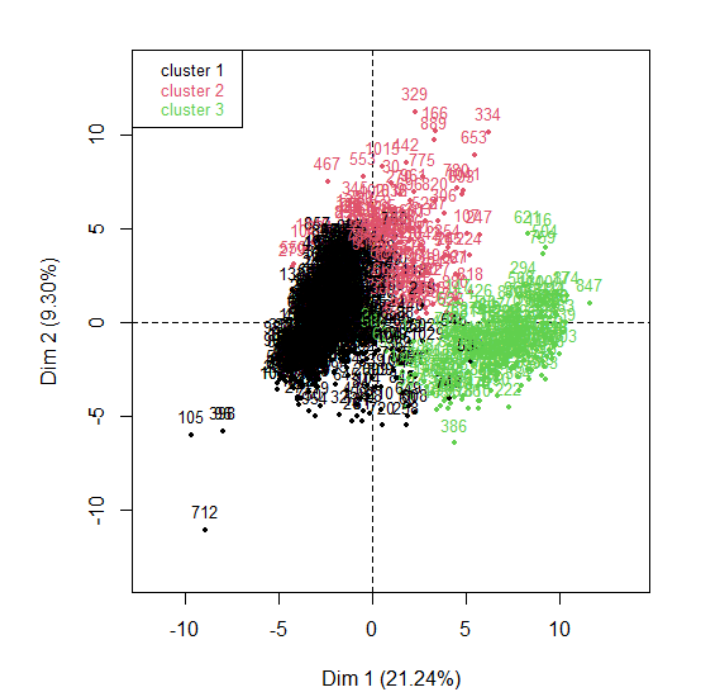
\includegraphics[scale=0.7]{classification_2.png} 
\caption[]{Ascending \ Hierarchical \ Classification \ of \ the \ individuals }
\end{center}
\end{figure}

\begin{figure}[H]
\begin{center}
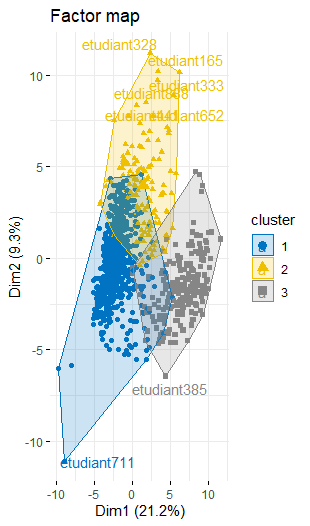
\includegraphics[scale=0.8]{hcpc.png} 
\caption[]{Ascending \ Hierarchical \ Classification \ of \ the \ individuals }
\end{center}
\end{figure}


\subsection{Results of HCHC}

Cluster 1 consists of individuals sharing:
\begin{itemize}
    \item  high values for the variables Galbant, Culpability, Boredom, 
Stretching, Security, Discouragement, Slowness, Lassitude,
Discomfort, and Passivity (variables are sorted from the highest).  
    
    \item  low values for variables such as Progression, Perspiration, Performance,
Active, Challenge, Fun, Goal, Perseverance, Self-confidence and Cardio 
(the variables are sorted from the lowest).

\end{itemize}

Cluster 2 consists of individuals who share:


\begin{itemize}
    \item High values for variables such as Blast Off, Power, Competition, Technicality, Quality, Energy, Comfort, Muscle, Strength, and Intensity (variables are sorted from highest).
    \item Low values for the variables Sexy, Best, Calm and Vital (the variables are sorted from the lowest).
\end{itemize}

Cluster 3 consists of individuals who share:

\begin{itemize}
    \item High values for variables such as Progression, Active, Performance, Challenge, Cardio, Sharing, Fun, Overcoming, Fast, and Efficiency (variables are sorted from highest).

    \item Low values for variables such as Comfort, Safety, Shaping, Softness, Boring, Strength, Holding, Quality, Beauty and Discomfort (variables are sorted from the lowest).

\end{itemize}


\section{Classification}  %%%%  Testing the strength of clusters %%%%
 
 We separated our data in 2 parts: 80 \% of the data for the choice of the selection algorithm,20 \% of the data to test the final model and eventually select the most important columns.
 
 
\subsection{Choice of Classification algorithm} 

 4 multi-class classifiers are used: the support vector classifier
(SVC), linear support vector classifier
(LSVC), k-nearest neighbors (KNN) and logistic regression (logreg). 
(KNN) and logistic regression (logreg).

\vspace{0.4 cm}

Here is the graph of the performance of each model: 


\begin{figure}[H]
\begin{center}
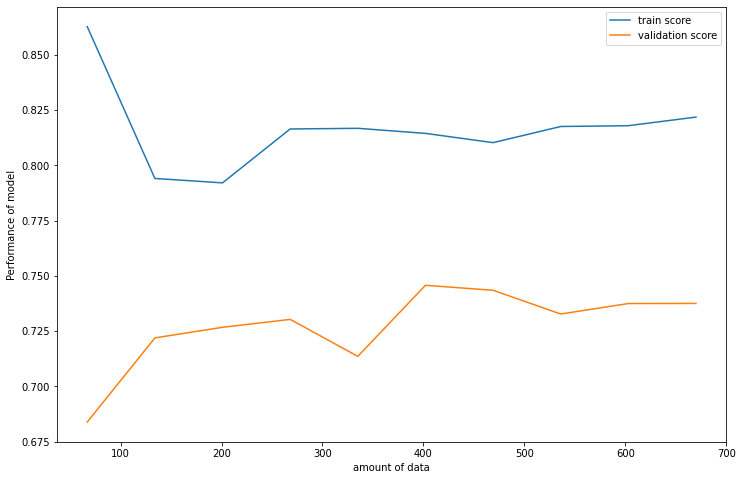
\includegraphics[scale=0.6]{learning_curve_1.png} 
\caption[]{ KNN \ learning \ curve }
\end{center}
\end{figure}

\begin{figure}[H]
\begin{center}
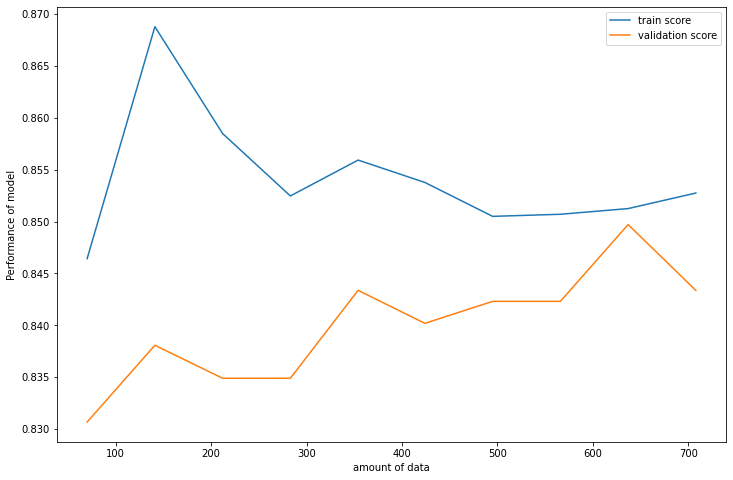
\includegraphics[scale=0.6]{learning_curve_2.png} 
\caption[]{ logreg \ learning \ curve }
\end{center}
\end{figure}

\begin{figure}[H]
\begin{center}
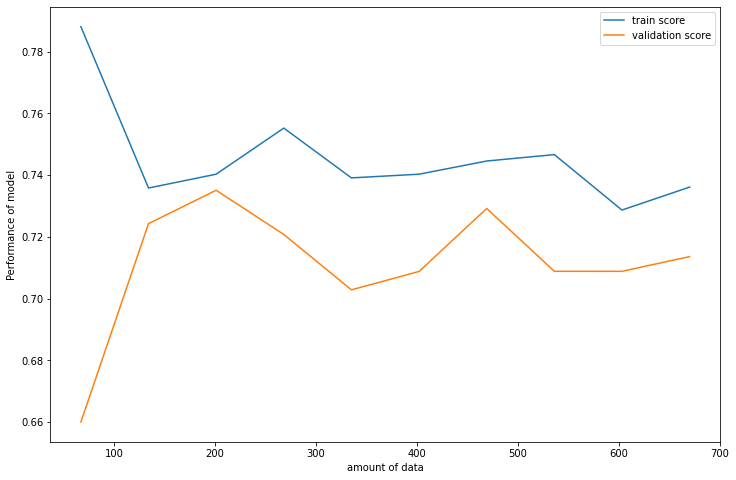
\includegraphics[scale=0.6]{learning_curve_3.png} 
\caption[]{ LSVC \ learning \ curve }
\end{center}
\end{figure}

\begin{figure}[H]
\begin{center}
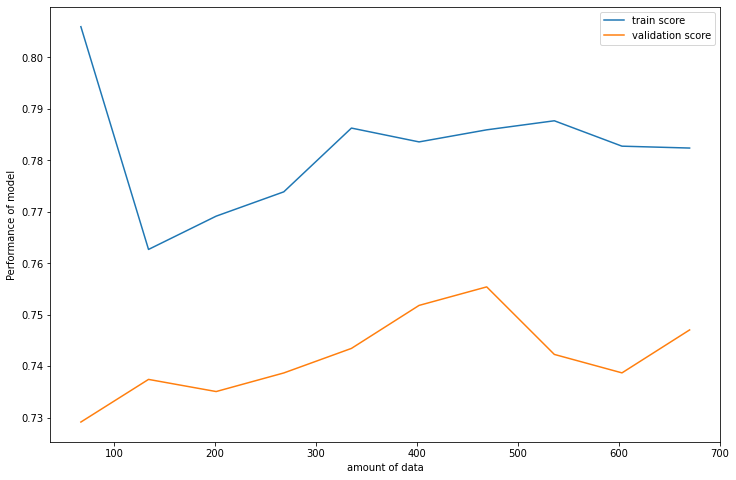
\includegraphics[scale=0.6]{learning_curve_4.png} 
\caption[]{ SVC \ learning \ curve }
\end{center}
\end{figure}


According to the graphs below, the performance of the lostigic Regression and SVC models is more stable and better than the other models. We can say that the two models are not overfitting
(train score and val score are close) contrary to the other two models.

\vspace{0.2 cm}

Nous avons utlisé  GridSearchCV pour optimser les hyperparametres du modele  logistic Regression. 
GridSearchCV nous permet de les meilleurs hyperpametre en comparant les différents performances 
 de chaque combinaison grâce a la technique de cross-validation.
 
\vspace{0.2 cm}

We used GridSearchCV to optimize the hyperparameters of the logistic Regression model. 
GridSearchCV allows us to select the best hyperparameters by comparing the different performances of each 
 of each combination using the cross-validation technique.

  
\subsection{Feature selection} 


\noindent The graph below shows the variance of each feature. 
 4 threshold candidates stand out: 0.8, 0.06, 0.04 and 0.02.



\begin{figure}[H]
\begin{center}
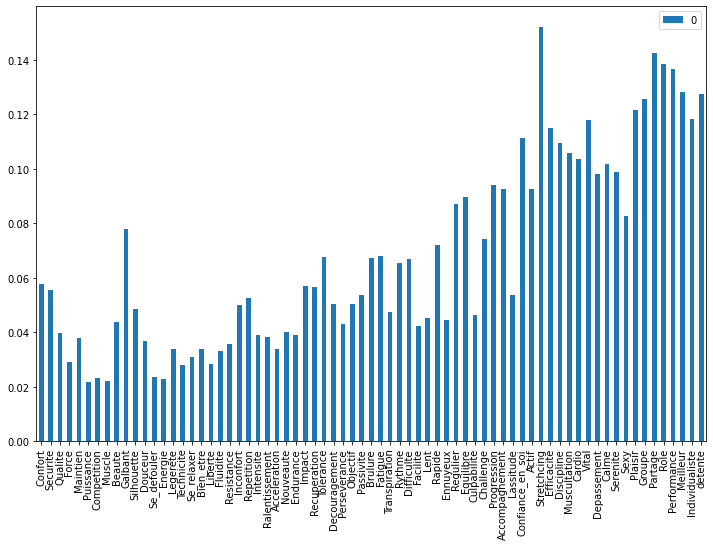
\includegraphics[scale=0.6]{barlot.png}
\caption[]{ variance\ of \ each \ features}
\end{center}
\end{figure}

\noindent To eliminate the values below this threshold, the VarianceThreshold function of scikit-learn is used.In the end, the threshold set at 0.02 gives better results. No column was suppressed. 

\subsection{Results final model} 

\begin{figure}[H]
\begin{center}
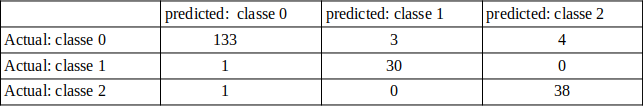
\includegraphics[scale=0.6]{confusion_matrix_1.png} 
\caption[]{ confusion \ matrix }
\end{center}
\end{figure}



\begin{figure}[H]
\begin{center}
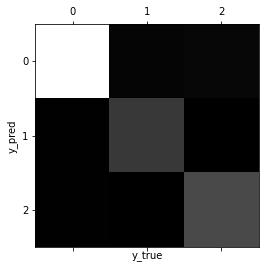
\includegraphics[scale=0.6]{confusion_matrix_2.png} 
\caption[]{ image of confusion matrix  }
\end{center}
\end{figure}

\noindent We obtain satisfactory results: 
only 9 misplaced values, the value of 0.964 and 0.94768 for the recall\_score and the f1\-score.

\section{Conclusion}
The main objective of the project was to do clustering on our data.
Thanks to the HCPC clustering, we can distinguish 3 types of students:

\begin{itemize}

\item The unmotivated, those who seek well-being and simplicity, whose characteristic variables of the cluster are:  Guilt, Boredom, Discouragement, Slowness, Discomfort 

\item In the second group, we have those who like combat sports such as wrestling, boxing and MMA. It is characterized by its words: Power, Competition, Technicite, Qualite, Energie, Muscle, Force and Intensite 

\item  The last group is characterized by its words: Progression, Performance, 
Challenge, Cardio, Sharing, Exceeding, Fast and Efficiency. 
We find those who enjoy running and nature activities. 

\end{itemize}

\noindent Regarding classification, one of the best algorithms (SVM) gave the value of 0.9549 of precision,0.9 of recall and 0.9255 of f1-score.


\begin{thebibliography}{9}

\bibitem{text}
\url{https://www.cairn.info/revue-staps-2018-2-page-99.htm}

\bibitem{text}

\url{https://solidarites-sante.gouv.fr/prevention-en-sante/preserver-sa-sante/article/activite-physique-et-sante}

\bibitem{text}
\url{https://e3s.unistra.fr/equipe/presentation/}

\bibitem{text}
\url{https://scikit-learn.org}

\bibitem{}
\url{https://fr.wikipedia.org/wiki/Analyse_en_composantes_principales}


\bibitem{text}
\url{http://www.sthda.com/english/}

\bibitem{text}
\url{http://www.sthda.com/english/articles/31-principal-component-methods-in-r-practical-guide/117-hcpc-hierarchical-clustering-on-principal-components-essentials/#algorithm-of-the-hcpc-method}


\bibitem{text}
\url{https://husson.github.io/teaching.html}


\bibitem{text}
\url{https://www.youtube.com/c/MachineLearnia}



\end{thebibliography}



\end{document}

